\documentclass[10pt]{beamer}
\usetheme[
%%% option passed to the outer theme
%    progressstyle=fixedCircCnt,   % fixedCircCnt, movingCircCnt (moving is deault)
  ]{Feather}
  
% If you want to change the colors of the various elements in the theme, edit and uncomment the following lines

% Change the bar colors:
%\setbeamercolor{Feather}{fg=red!20,bg=red}

% Change the color of the structural elements:
%\setbeamercolor{structure}{fg=red}

% Change the frame title text color:
%\setbeamercolor{frametitle}{fg=blue}

% Change the normal text color background:
%\setbeamercolor{normal text}{fg=black,bg=gray!10}

%-------------------------------------------------------
% INCLUDE PACKAGES
%-------------------------------------------------------

\usepackage[utf8]{inputenc}
\usepackage[english]{babel}
\usepackage[T1]{fontenc}
\usepackage{graphicx}
\usepackage{helvet}


%-------------------------------------------------------
% DEFFINING AND REDEFINING COMMANDS
%-------------------------------------------------------

% colored hyperlinks
\newcommand{\chref}[2]{
  \href{#1}{{\usebeamercolor[bg]{Feather}#2}}
}

%-------------------------------------------------------
% INFORMATION IN THE TITLE PAGE
%-------------------------------------------------------

\title[] % [] is optional - is placed on the bottom of the sidebar on every slide
{ % is placed on the title page
      \textbf{CI/CD}
}

\subtitle[Descomplicando o CI/CD]
{
      \textbf{CI/CD}
}

\author[Eugenio Cunha]
{      Eugenio Cunha
      {}
}

\institute[]
{
      TWT Info
  %there must be an empty line above this line - otherwise some unwanted space is added between the university and the country (I do not know why;( )
}

\date{\today}

%-------------------------------------------------------
% THE BODY OF THE PRESENTATION
%-------------------------------------------------------

\begin{document}

%-------------------------------------------------------
% THE TITLEPAGE
%-------------------------------------------------------

% {\1% % this is the name of the PDF file for the background



\begin{frame}{Descomplicando o CI/CD}{}
    \begin{center}
        
\includegraphics[scale=0.3]{images/cicd}
    \end{center}
\end{frame}

\section{Content}

%-------------------------------------------------------
\subsection{Descomplicando o CI/CD}
\begin{frame}{Conteúdo}{Descomplicando o CI/CD}
  \begin{itemize}
    \item O que é CI/CD?
    \item CI/CD é um Hype das tecnologias emergentes?
    \item CI/CD é cultura DevOps?
    \item Exemplo de CI/CD.
  \end{itemize}
\end{frame}
%-------------------------------------------------------

%-------------------------------------------------------
\section{Introduction}
\subsection{Descomplicando o CI/CD}
\begin{frame}{O que é CI/CD?}{Descomplicando o CI/CD}
  \begin{center}
    
\includegraphics[scale=0.38]{images/acdc.png}
  \end{center}
   \begin{center}
      Não é uma banda de rock'n'roll! Eles são AC/DC.
   \end{center}
\end{frame}
%-------------------------------------------------------

%-------------------------------------------------------
\section{Introduction}
\subsection{Descomplicando o CI/CD}
\begin{frame}{O que é CI/CD?}{Descomplicando o CI/CD}
    \begin{center}
      O que é CI/CD? \\~\\ ``De forma resumida, é automatizar o processo de entrega de software de forma rápida, ou melhor, continua, sem perder a qualidade.''
    \end{center}
\end{frame}
%-------------------------------------------------------

%-------------------------------------------------------
\section{Introduction}
\subsection{Descomplicando o CI/CD}
\begin{frame}{O que é CI/CD?}{Descomplicando o CI/CD}
    \begin{center}
      O que CI? \\~\\ ``CI ou Integração contínua, nada mais é que: compilar e testar software toda vez que um desenvolvedor envia código para o repositório, de forma automatizada, várias vezes ao dia.''
    \end{center}
\end{frame}
%-------------------------------------------------------

%-------------------------------------------------------
\section{Introduction}
\subsection{Descomplicando o CI/CD}
\begin{frame}{O que é CI/CD?}{Descomplicando o CI/CD}
    \begin{center}
      O que CD? \\~\\ ``CD ou Entrega contínua, nada mais é que: entrega automatizada de forma rápida, confiável, repetitiva e com o mínimo de intervenção humana!''
    \end{center}
\end{frame}
%-------------------------------------------------------

%-------------------------------------------------------
\section{CICD}
\subsection{Descomplicando o CI/CD}
\begin{frame}{O que é CI?}{Descomplicando o CI/CD}
  \begin{center}
    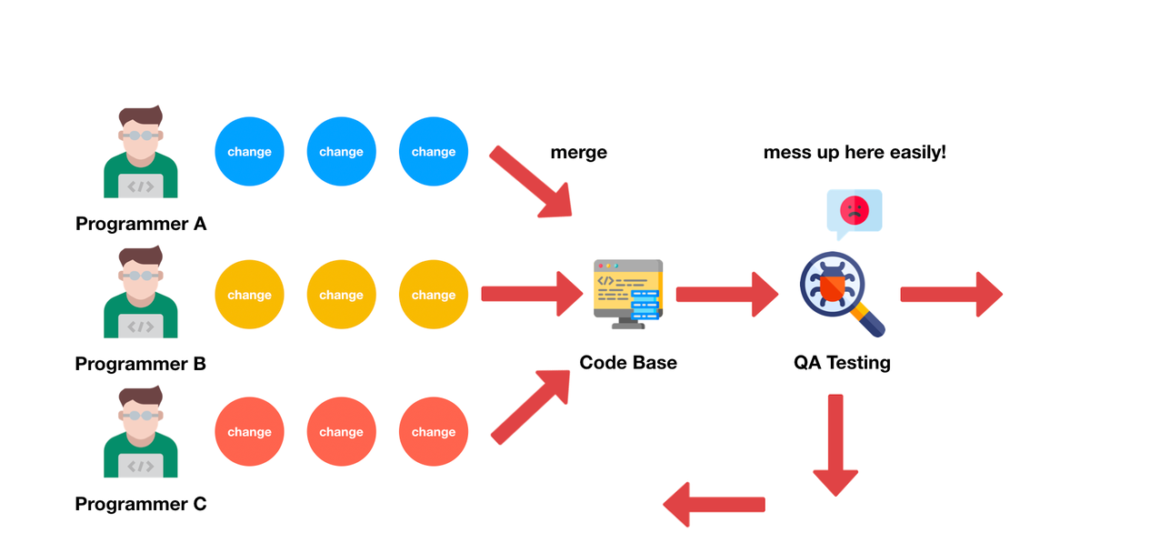
\includegraphics[scale=0.25]{images/traditional.png}
  \end{center}
  \begin{center}
      Desenvolvimento de software tradicional.
   \end{center}
\end{frame}
%-------------------------------------------------------

%-------------------------------------------------------
\section{CICD}
\subsection{Descomplicando o CI/CD}
\begin{frame}{O que é CI/CD?}{Descomplicando o CI/CD}
  \begin{center}
    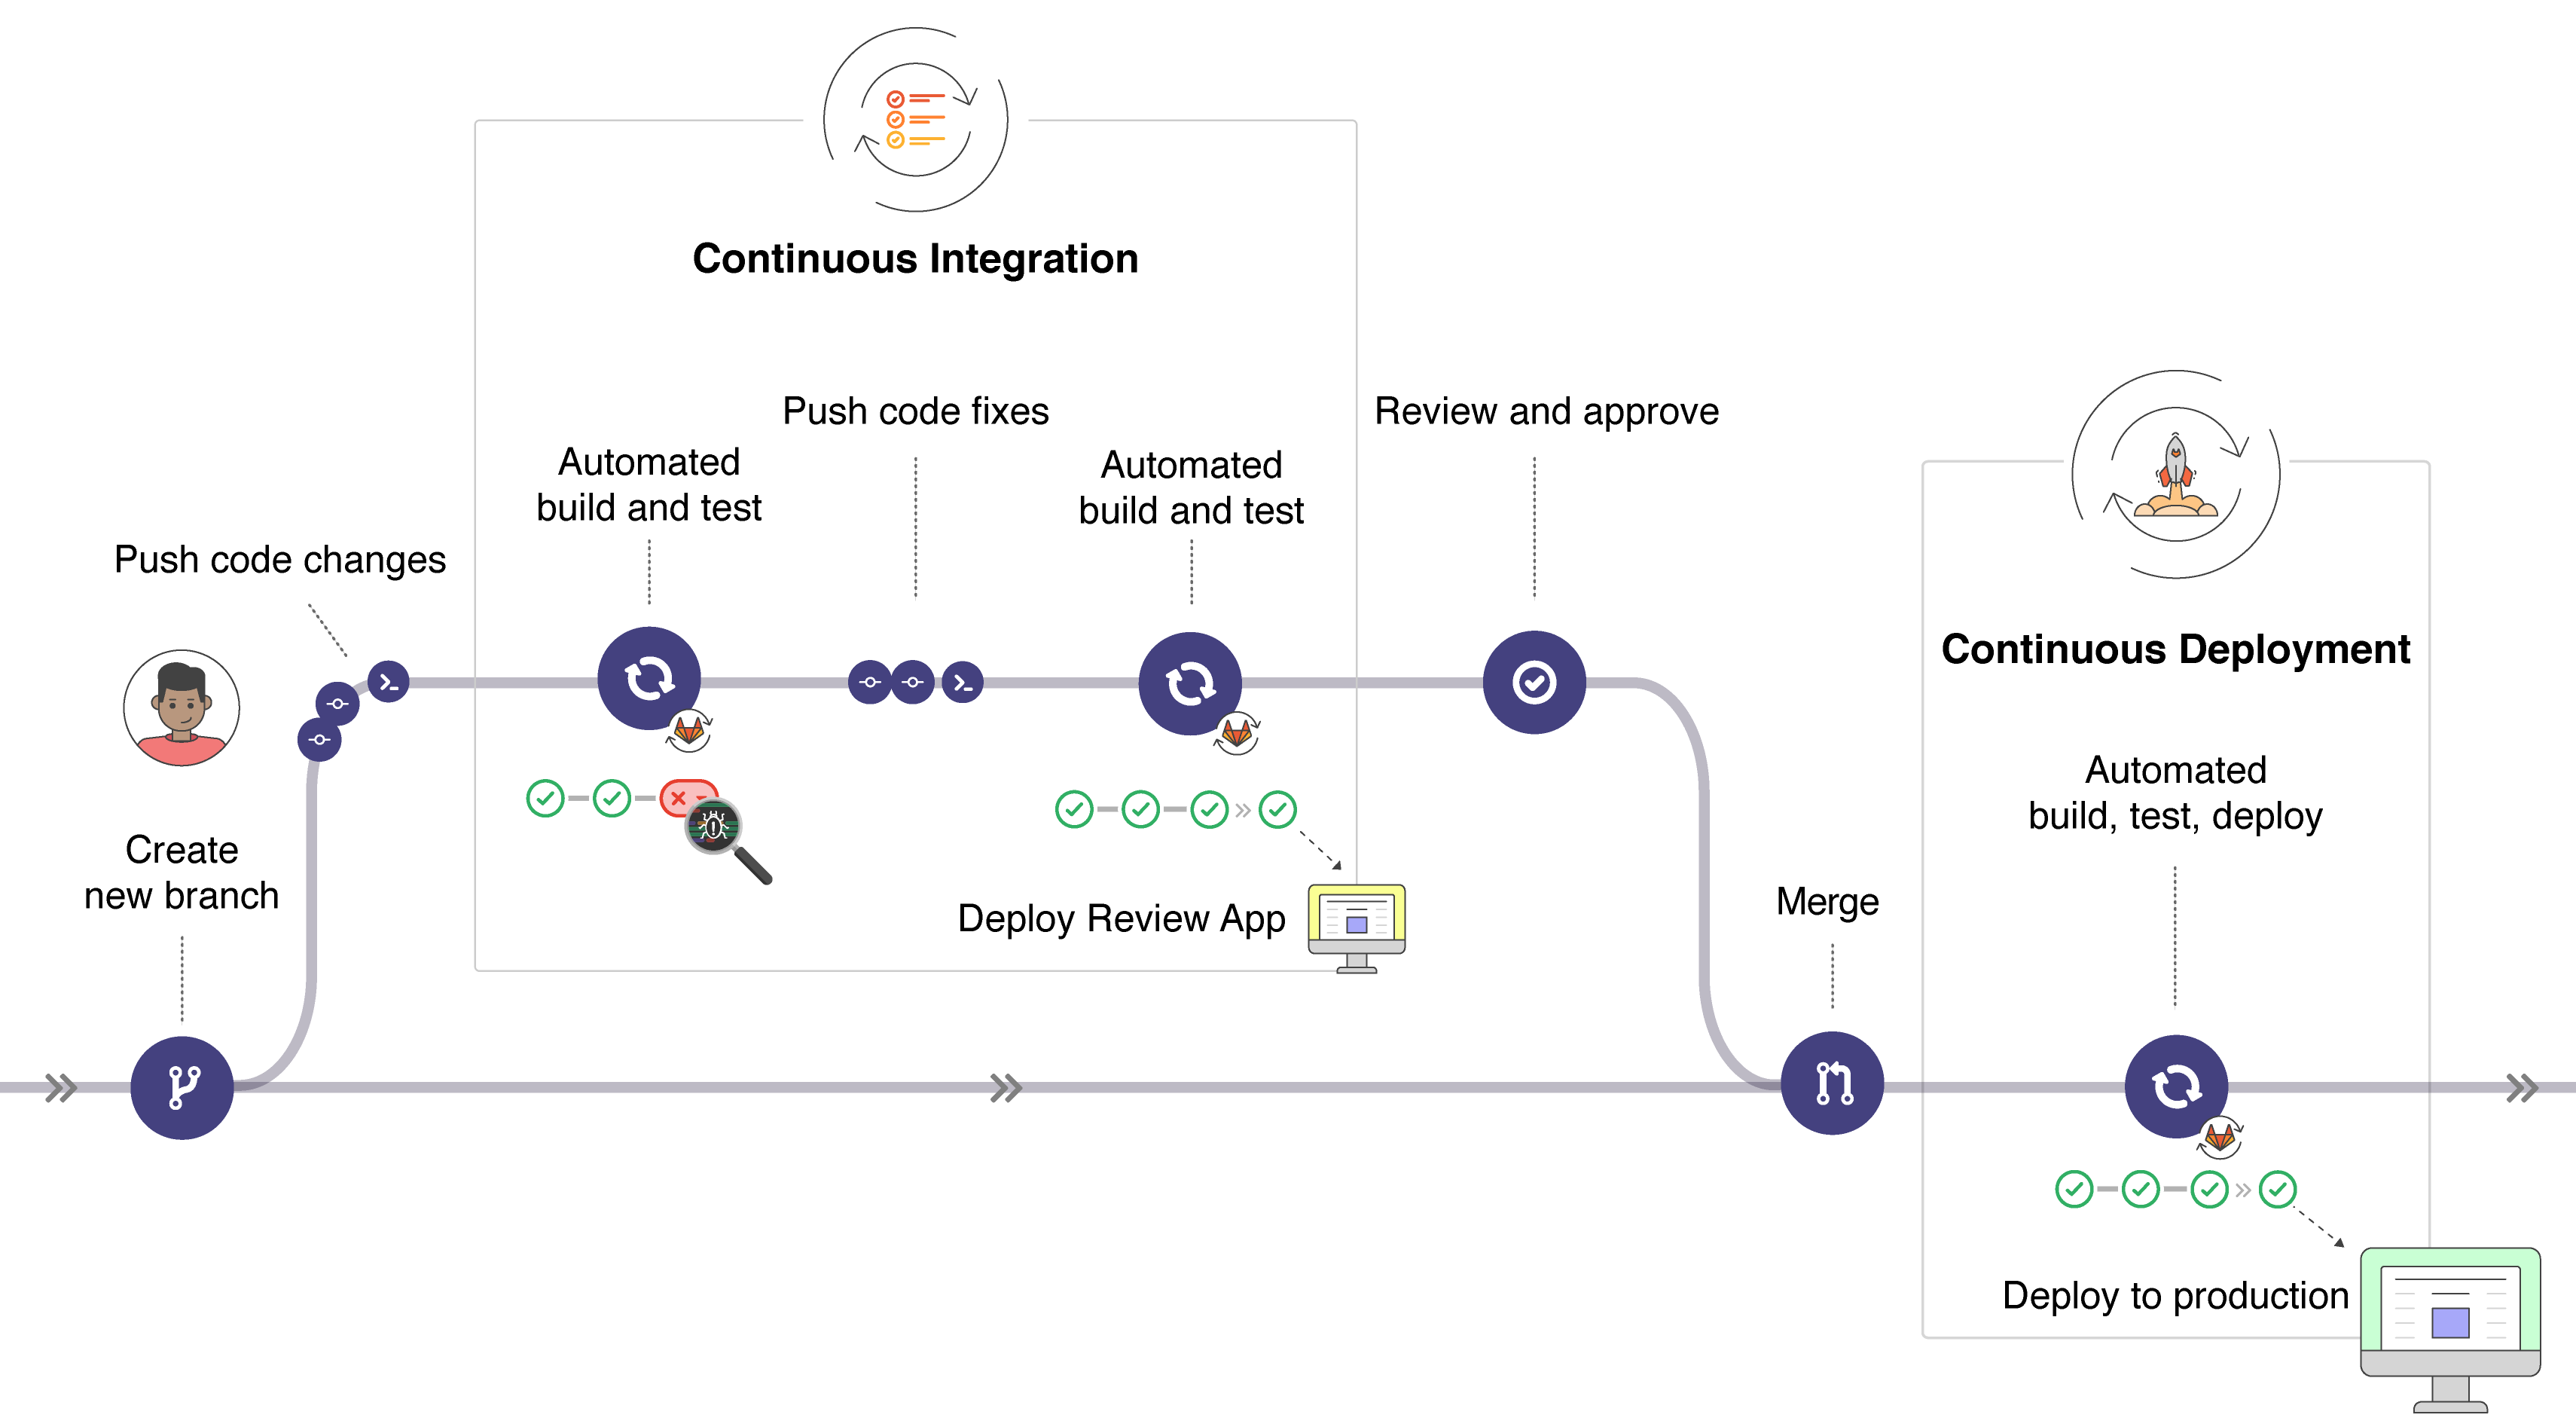
\includegraphics[scale=0.09]{images/workflow.png}
  \end{center}
  \begin{center}
      Desenvolvimento de software com um pipeline para CI\textbackslash CD.
   \end{center}
\end{frame}
%-------------------------------------------------------

%-------------------------------------------------------
\section{HYPE}
\subsection{Descomplicando o CI/CD}
\begin{frame}{CI/CD um Hype da tecnologia?}{Descomplicando o CI/CD}
    \begin{center}
     
\includegraphics[scale=0.25]{images/hype.png}
    \end{center}
\end{frame}
%-------------------------------------------------------

%-------------------------------------------------------
\section{DEVOPS}
\subsection{Descomplicando o CI/CD}
\begin{frame}{CI/CD é parte da cultura DevOps?}{Descomplicando o CI/CD}
    \begin{center}
     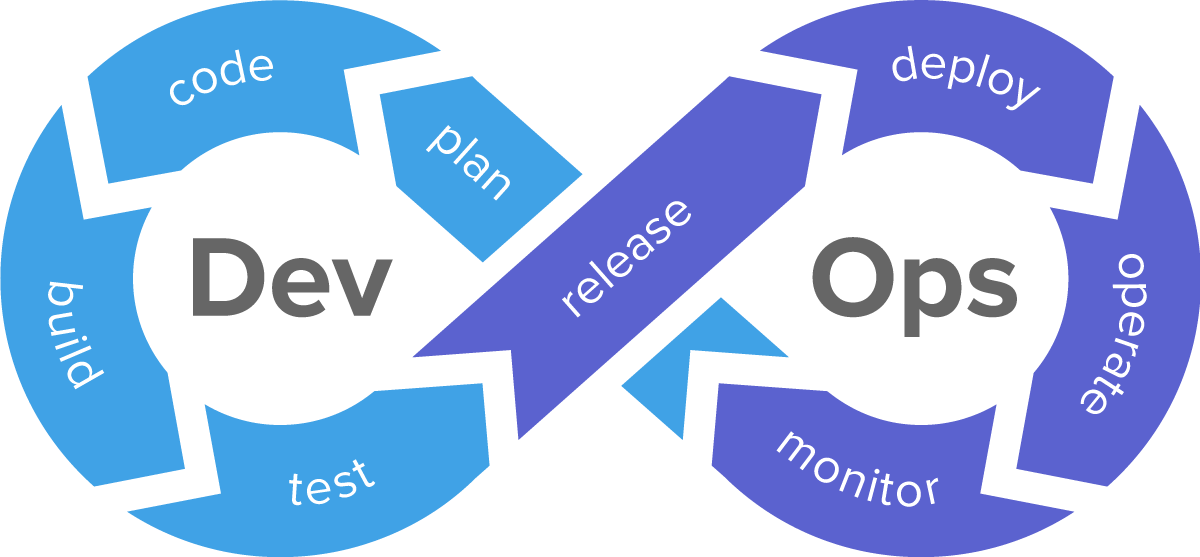
\includegraphics[scale=0.25]{images/devops}
    \end{center}
\end{frame}
%-------------------------------------------------------

%-------------------------------------------------------
\section{Tools}
\subsection{Descomplicando o CI/CD}
\begin{frame}{Ferramentas CI/CD}{Descomplicando o CI/CD}
\begin{table}[]
\begin{tabular}{|l|c|c|c|c|c|}
\hline
               & \multicolumn{1}{l|}{Open} & \multicolumn{1}{l|}{Grátis} & \multicolumn{1}{l|}{GIT} & \multicolumn{1}{l|}{Pipeline} & \multicolumn{1}{l|}{Infra Interna} \\ \hline
www.gitlab.com & \checkmark                       & \checkmark                         & \checkmark                      & \checkmark                           & \checkmark                                \\ \hline
www.github.com & -                       & \checkmark                         & \checkmark                      & \checkmark                           & -                                \\ \hline
www.jenkins.io & \checkmark                       & \checkmark                         & -                      & \checkmark                           & \checkmark                                \\ \hline
\end{tabular}
\end{table}
\end{frame}
%-------------------------------------------------------

%-------------------------------------------------------
\section{Sample}
\subsection{Descomplicando o CI/CD}
\begin{frame}{Show me the code}{Descomplicando o CI/CD}
    \begin{center}
    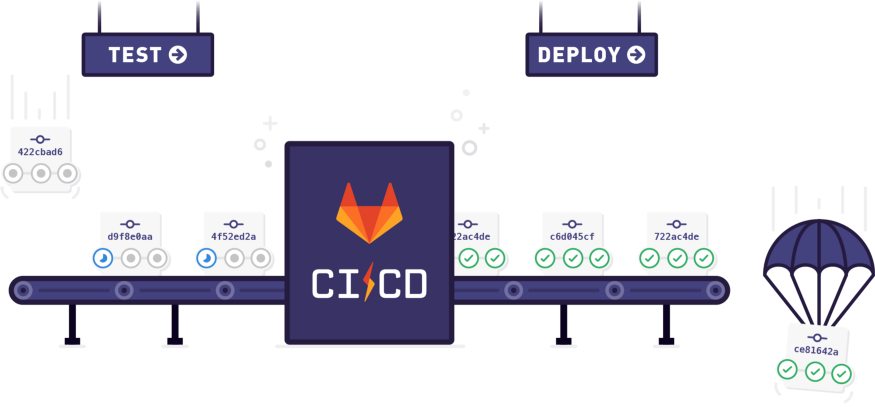
\includegraphics[scale=0.3]{images/gitlab.png}
    \end{center}
\end{frame}
%-------------------------------------------------------

{\1
\begin{frame}[plain,noframenumbering]
  \finalpage{www.eugenio.xyz \\~\\ https://github.com/eugenio-cunha/cicd \\~\\ Thank you! ;) }
\end{frame}}

\end{document}